\index{Schwender, Clemens}

\paragraph{Research Team}
Clemens Schwender (Professor), Christoph K\"{o}hler (Dipl. Media Consultant), Ulrich B\"{u}hring (Student Assistant Donau University Krems).

 In our homes and at work we are confronted with new technology. Written, AV- or online-documentations explain how to build or handle these artefacts. Again and again we are faced with situations in which technology is not self-explaining but needs introduction instead. Media-based teaching happens without the presence of a teacher. People must read and understand text and pictures. Formatting and design play crucial roles in the motivation to access user's manuals. There is no option of asking questions and receiving immediate answers. Manuals must reflect the restrictions and preferences of the users of different age, gender and cultural background.

\begin{figure}[h]
  \begin{center}
    \begin{minipage}[b]{0.35\linewidth}
   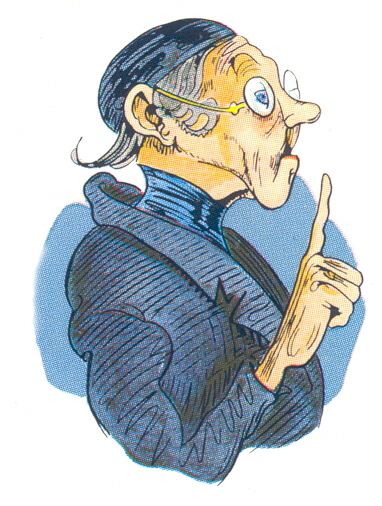
\includegraphics[width=\linewidth]{profClemensSchwender-fig1.jpg}
    \end{minipage}\hfill
    \begin{minipage}[b]{0.55\linewidth}
      \caption{Taken from Wilhelm Busch (1865): Max und Moritz. This kind of humorous dispersal is not accepted in technical documentation.\label{fig1:profClemensSchwender}}
    \end{minipage}
  \end{center}
\end{figure}

 Technical documentation is usually associated with boring reading. People avoid taking the manuals in their hands. We are investigating how motivation can be improved by making changes in the design: The page layout, font type and font size are considered as well as the use of more pictures and pictures that portrait not only machines but also people. The role of humor will be tested, to see if it has an influence on the motivation to look at a manual and to read it.

\null
\textbf{Research Highlights 2006}

 The research on technical documentation is a prototype for learning in adulthood. Technical documentation is an important example of lifelong learning. We try to observe how the learning process takes place without the presence of a teacher. In our working group we look at the formatting of information and test different conditions with persons of different age. 

 First results indicate that color and font size play a positive role and can be considered as motivational factors. Humor and comic-style pictures provoke resistance against the documentation. Effects on the speed of transforming reading into action and the accuracy of accomplishment cannot be found.


\paragraph{Collaborations}
\begin{itemize}
\item tekom - Der deutsche Fachverband f\"{u}r Technische Kommunikation und Informationsentwicklung
\end{itemize}

\begin{bibunit}[apalike]
\nocite{*}
\putbib[profClemensSchwender2]
\end{bibunit}